\chapter{Experiments and Results}
\addcontentsline{toc}{chapter}{Experiments and results}

\section{Experimental Setup}
	Thanks to the configurability of the programme the majority of experiments were run in a batch processing mode. That is a script in bash was written that allowed running multiple tests in series without any maintenance from the user. In a single series of tests any parameters could be modified or any data processing algorithm could be exchanged. All experiments were run on a notebook with Intel Core i7 quad core 2.2 GHz CPU, 8 GB of RAM and a nVidia M540 GPU.

\section{Experiments}
	The Bag of Words classification pipeline consists of four previously discussed steps. For there are many different algorithms suitable for each part of the pipeline, an extensive research is required in order to discover the best possible combination in a particular setting. The number of options grows combinatorial with number of candidates for each processing step. Moreover, many algorithms have different parameters that should be adjusted for any given conditions. Evaluation of every possibility is unfeasible due to the lack of time and computational power required. Even if only a single library, PCL, is considered, there are far too many options with 12 keypoint detectors and more than 20 feature description algorithms. 
	
	\subsection{Detectors}
	In a paper \cite{pcl_keypoint_comparision} some keypoint detection algorithms from PCL are evaluated. It is stated that , albeit under slightly different conditions, the SIFT and ISS keypoint detectors achieve the highest performance. Therefore this paper compares only these two modules with respect to their usability in the BoW pipeline. 

	\subsection{Descriptors}
	Recently a PCL's descriptors evaluation was performed in \cite{pcl_features}. The PFHRGB and SHOTCOLOR scored best. Only a little bit worse were PFH, FPFH, SHOT and USC. In this paper FPFH, PFH and PFHRGB are compared, motivation being that PFH is the original descriptor, FPFH is its approximate and thus faster version, while PFHRGB is an extension which makes use of colour information.
	
	\begin{table}[!ht]
	\centering	
	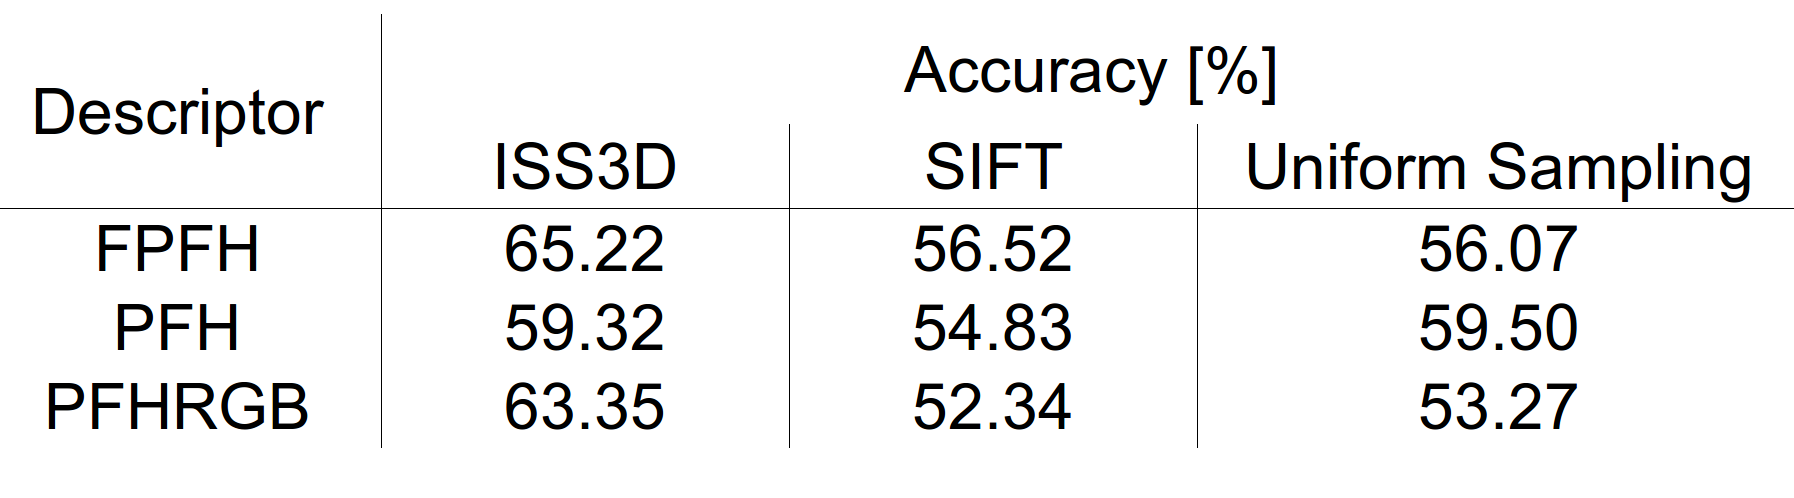
\includegraphics[width=.25\textwidth]{figs/desc_b3do}
	\caption{Highest accuracy obtained with FPFH, PFH and PFHRGB descriptors on the B3DO dataset}
	\label{tab:desc_b3do}
	\end{table}
	
	The figure \ref{tab:desc_b3do} shows highest accuracy obtained with the tested descriptors on the B3DO dataset. FPFH scored the best result, even tough it is an approximate and theoretically the least precise of all evaluated descriptors. On the other hand, the PFHRGB scored better than PFH. It does not surprise, since the colour information is believed to have discriminative value.
		
	\subsection{Codebook}
	KMeans is used in almost every implementation of the Bag of Words image processing pipeline \cite{tsai2012bag, toldo2009bag}. Csurka \emph{et al} showed that the number of visual words or centroids have a significant impact on the final results \cite{csurka2004visual}. Therefore a number of tests were run in order to determine the optimal dictionary size.
	
	\begin{figure}[!ht]
	\centering	
	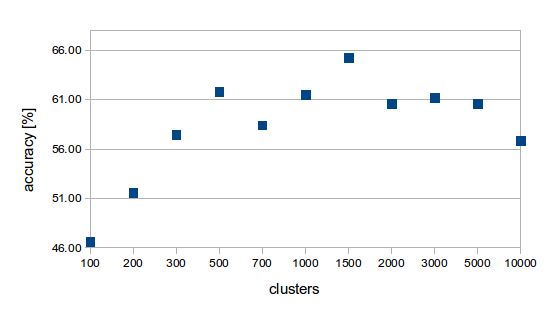
\includegraphics[width=.75\textwidth]{figs/clustering_centroids_b3do}
	\caption{Influence of dictionary size on the overall accuracy. B3DO dataset with ISS keypoint detector and FPFH feature descriptor}
	\label{fig:cluster_b3do}
	\end{figure}
	
	The results from the figure \ref{fig:cluster_b3do} partially confirm Csurka's findings. The performance raises with the increasing number of centroids up to the point of 1500 centroids and 65.22\%. Then it starts to diminish. The discrepancy might be caused by the following factors: (1) ISS detector finds too many or irrelevant points, thus introducing noise or (2) The FPFH descriptor has too few dimensions (33) to be divided into more than 1500 regions in a meaningful way. 

	
	\subsection{B3DO}
	Extraction of single objects yielded 78 separate categories with number of entries ranging from 1 (tape) to 299 (table). 8 categories were picked at random with a restriction that there should be at least 50 instances in each of them. Further, the objects were split into two sets (training and testing) with a proportion of 1:1. As names suggest, the estimation is performed on the test set and the evaluation on the test set.
	
	The highest accuracy achieved for this dataset is 64\%. Table \ref{tab:b3do_conf_matrix} contains a confusion matrix, number of examples per category and accuracy. The confusion matrix depicts misclassification errors. Let m\subscript{i, j} be an element of the confusion matrix at the i\superscript{th} row and j\superscript{th} column. It shows how many elements from the i\superscript{th} category was assigned to the j\superscript{th} category. A high value of m\subscript{i, j} such that $i \neq j$ indicates that the classifier cannot distinguish between those two classes.
	
	\begin{table}[!ht]
	\centering
	\caption{Results on the B3DO dataset with ISS keypoint detector, FPFH features and a dictionary of 1500 words. \textbf{Overall accuracy is 65.22\%}}
	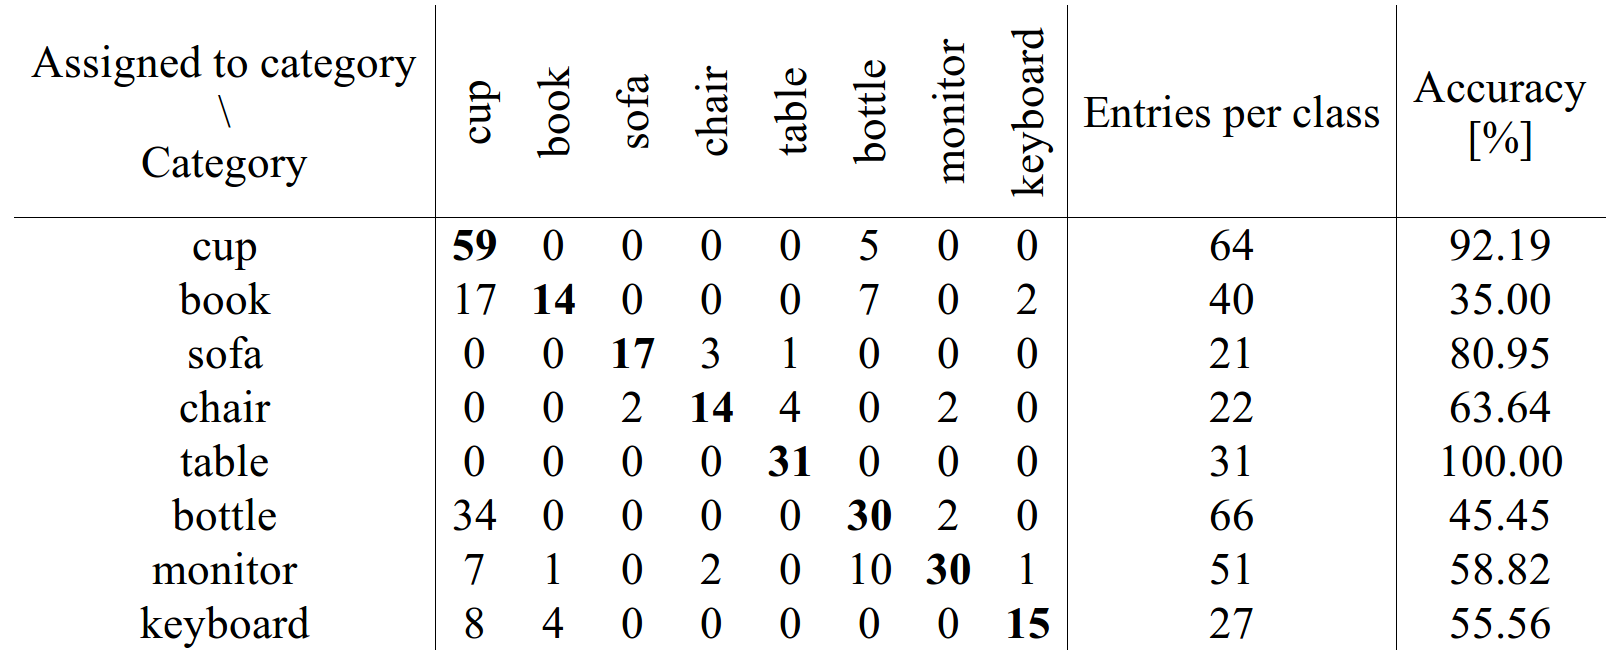
\includegraphics[width=0.9\textwidth]{figs/b3do_conf_matrix}	
	\label{tab:b3do_conf_matrix}
	\end{table}
	
	\begin{figure}[!ht]
	\centering	
	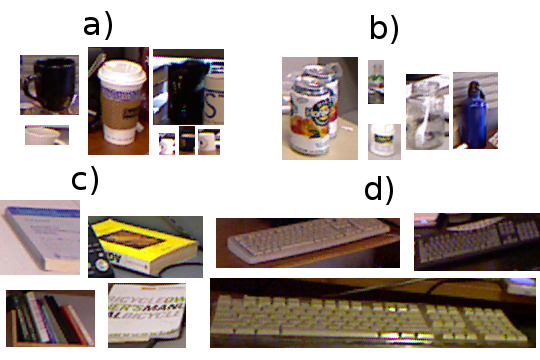
\includegraphics[width=.75\textwidth]{figs/b3do_objects}
	\caption{B3DO objects. Images are in their original sizes. a) cups b) bottles c) books d) keyboards}
	\label{fig:b3do_objects}
	\end{figure}
	
	More than half of the bottles were assigned to the cup category and keyboards were often mistook for books. These two error types are easily explained by a high degree of similarity of objects (bottles and cups are usually round and tall, books and keyboards are flat and rectangular) Surprisingly, however, objects from half of the categories were frequently marked as cups. Some of these misclassification errors might be caused by very poor quality of images. Many of them are occluded poorly lit low resolution images.	
	
	\subsection{Tokyo}
	\begin{table}[!ht]
	\centering
	\caption{Tokyo confusion matrix with ISS keypoint detector, PFH features and a dictionary of 3000 words}
	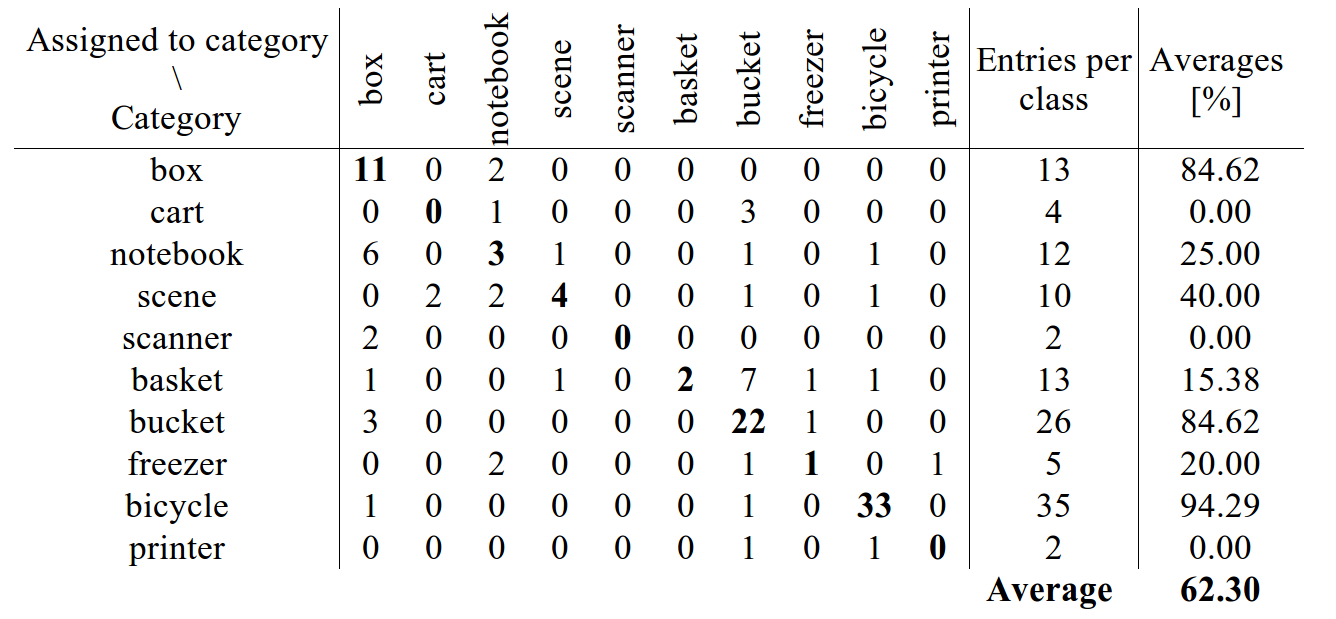
\includegraphics[width=0.9\textwidth]{figs/tokyo_conf_matrix}	
	\label{tab:tokyo_conf_matrix}
	\end{table}
	
	Every of the 343 images from Tokyo dataset was used. Data was split into test and train set in proportions 1:2 in order to provide more training examples due to low number of objects in some classes.
	
	Even tough the overall accuracy achieved on Tokyo dataset is similar in value to that of the B3DO, the structure of the result is very different. It is clearly visible that there is a strong correlation between a per class accuracy and the number of entries in this class. The highest performance in the bicycle category is coupled with the largest number of entries. On the other end of the scale there are cart and printer categories with only 2 and 4 entries respectively. On top of that there are differences between some classes are marginal. The majority of carts and baskets were put into the bucket category. It does not surprise, for they are simply akin as can be seen in figure \ref{fig:tokyo} on the page \pageref{fig:tokyo}.
	
\section{Conclusion}
	